% =====================================================================
% פרק 3 — מבוא היסטורי ב': שוק הדיור הישראלי 2022–2026
% Owner: Agent 1. Numbers aligned to comms/data_summary.json (verified points only)
% =====================================================================
\chapter{מבוא היסטורי ב׳: שוק הדיור בישראל, \en{2022–2026}}
\label{ch:israel}

\begin{managerbox}
בתוך ארבע שנים עבר שוק הדיור מריבית אפסית וביקושי שיא לריבית גבוהה, למלאי לא־מכור ברמת שיא ולשפל בעסקאות. היזמים הגיבו במבצעי מימון שהעבירו חלק מהסיכון אל העתיד. מנהל שמחליט על אשראי ליזם, על ליווי פרויקט או על רכישה במבצע ימצא כאן את העובדות ואת התגובה הרגולטורית שעליהן נשען ניתוח הסיכון בהמשך.
\end{managerbox}

\section{נקודת המוצא, הבלמים ומחזור הריבית}
\label{sec:ch3-baseline}

בעשור שקדם ל־\en{2022} שמר בנק ישראל על ריבית נמוכה מאוד, שירדה ל־\pct{0.10} בשנת \en{2020} \cite{boi_rate_decisions}. נוספו לכך מחסור מצטבר בדיור, הליכי תכנון ממושכים וריכוז הקרקע בידי המדינה \cite{boi_annual2025_housing}.

האשראי לדיור כפוף למגבלות מאקרו־יציבותיות שעוגנו בהוראה \en{329} \cite{boi_directive329}:
\begin{itemize}
  \item \textbf{שיעור מימון מרבי (\en{LTV}):} \pct{75} לרוכשי דירה יחידה, \pct{70} למשפרי דיור ו־\pct{50} למשקיעים.
  \item \textbf{יחס החזר מהכנסה (\en{PTI}):} עד \pct{50} מההכנסה, ומשקל סיכון מוגבר מעל \pct{40}.
\end{itemize}
לצד אלה פועלים \term{חוק המכר (דירות) (הבטחת השקעות של רוכשי דירות)}{Sale Law} \cite{salelaw1974}, המחייב את היזם להבטיח את כספי הרוכש, ומנגנון \term{הליווי הבנקאי הסגור}{Closed Project Finance}, שבו הבנק המלווה שולט בחשבון הפרויקט. בלמים אלה עומדים בבסיס \en{H3}, והם גם ההקשר ל־\en{H1}: מנגנון המאפשר לרוכש להתחייב לרכישה \textbf{לפני} שנבחן במגבלות פועל כעקיפה שלהן.

\paragraph{מחזור הריבית.}\label{sec:ch3-rates} באפריל \en{2022} החל בנק ישראל במחזור העלאות מהיר: בתוך \en{13} חודשים עלתה הריבית מ־\pct{0.10} ל־\pct{4.75}, וריבית הפריים, עוגן התמחור של רכיבי המשכנתא המשתנים, עלתה מ־\pct{1.60} ל־\pct{6.25}. לאחר הפחתה ל־\pct{4.50} בינואר \en{2024}, בצל לחצי האינפלציה ופרמיית הסיכון של המלחמה, החל בנובמבר \en{2025} מחזור של חמש הפחתות ברבע נקודה, עד \pct{3.25} (פריים \pct{4.75}) בספטמבר \en{2026} \cite{boi_rate_decisions,boi_rate_2026_09}; המסלול מוצג באיור~\ref{fig:inventory-rates}.

הריבית כרסמה בכוח הקנייה בעוד המחירים נותרו גבוהים, וכך נוצר הרקע למבצעי המימון.

\section{הביקוש, המחירים והמלאי הלא־מכור}
\label{sec:ch3-demand}

המלחמה שפרצה באוקטובר \en{2023} הוסיפה זעזוע היצע: הפסקת כניסתם של עובדים פלסטינים האריכה את משכי הבנייה וייקרה את עלויות היזמים \cite{boi_annual2025_housing}.

בשנת \en{2026} הפעילות בשוק חלשה: באפריל \en{2026} נרשמו \en{5,081} עסקאות בלבד \cite{semerenko_market}, ובאוגוסט \en{2026} נרשמו \en{7,532} \cite{toi_housing_2026_10}. באפריל ובמאי \en{2026} היה מדד מחירי הדירות נמוך ב־\pct{2.0} מרמתו שנה קודם \cite{cbs_priceindex_2026_222}, וביולי–אוגוסט \en{2026} ב־\pct{1.8} \cite{toi_housing_2026_10}. המדד מבוסס על המחיר המדווח, ולכן אינו משקף בהכרח את מלוא הירידה במחיר הכלכלי (\en{H1}).

\label{sec:ch3-inventory}לפי נתוני הלמ״ס, בינואר \en{2026} הגיע מלאי הדירות החדשות הלא־מכורות לשיא של \en{86,290} דירות \cite{cbs_newdwellings}, ובסוף ספטמבר \en{2026} עמד על \en{85,080} (\en{86,666} בניכוי עונתיות) \cite{cbs_newdwellings_2026q3}. איור~\ref{fig:inventory-rates} מציג יחד את הריבית, את המלאי ואת מספר העסקאות: המלאי קרוב לשיא גם לאחר ההפחתות.

\begin{figure}[!htb]
\centering
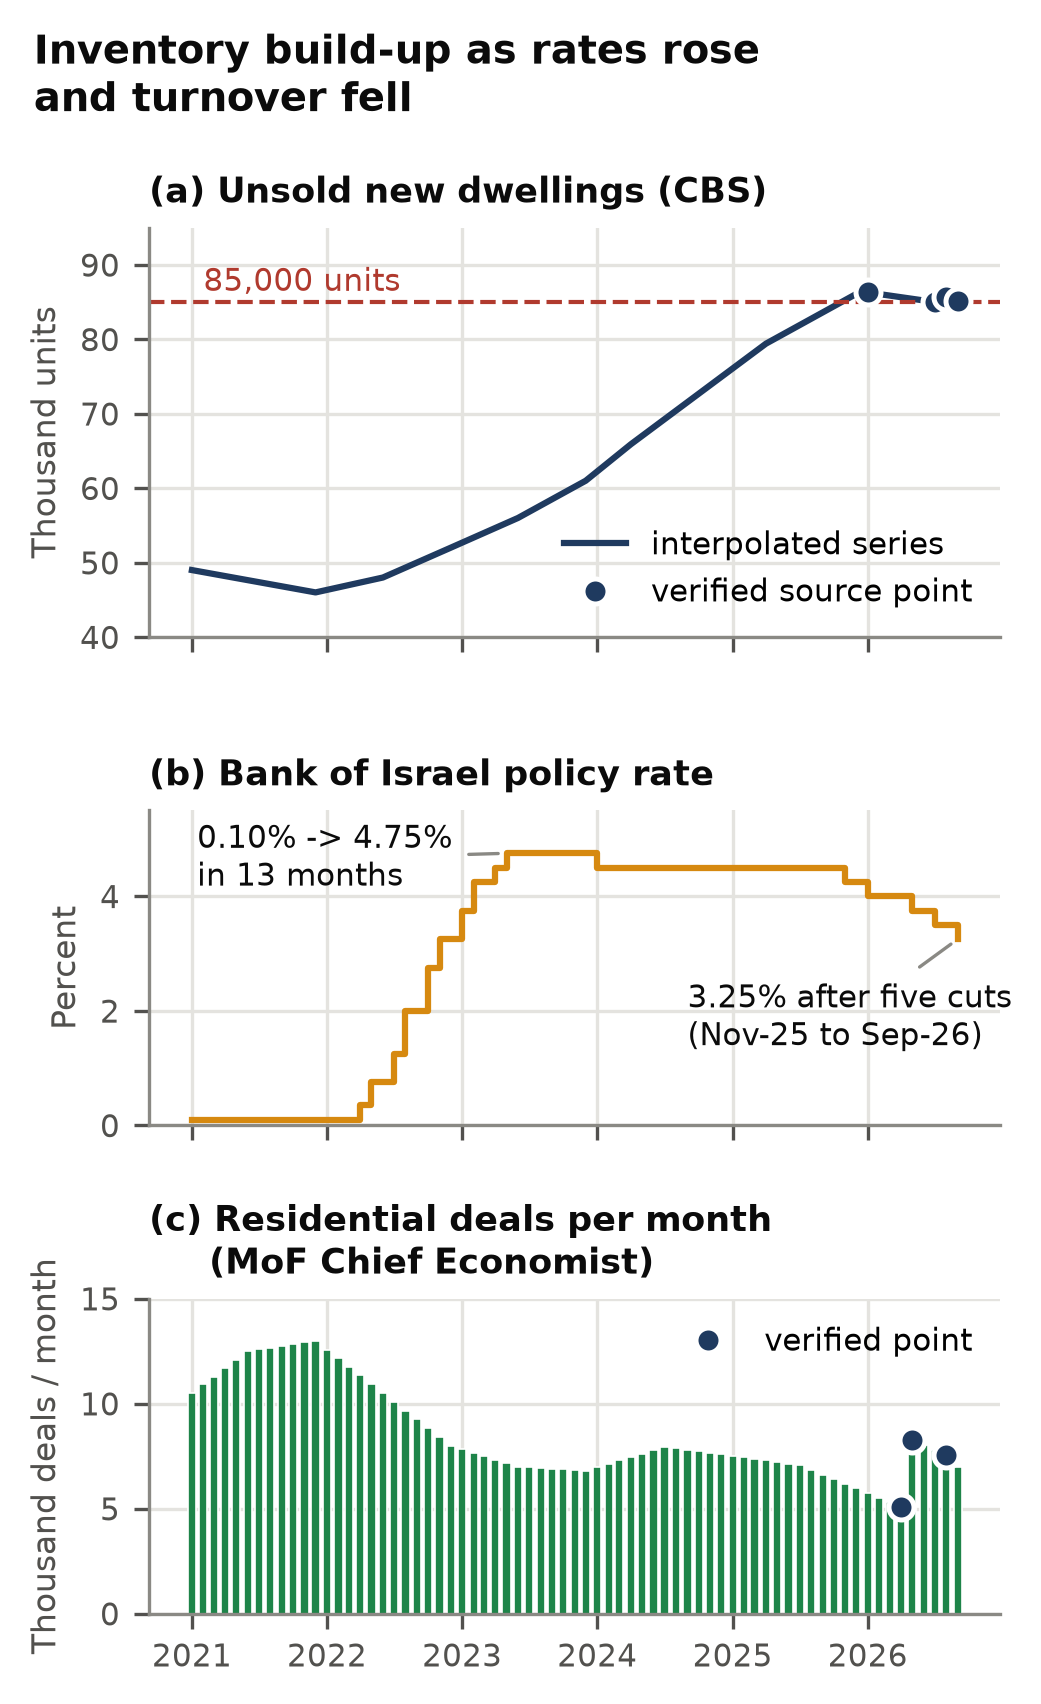
\includegraphics[width=0.6\textwidth]{figures/fig2_unsold_inventory_vs_rates.png}
\caption[מלאי לא־מכור, ריבית בנק ישראל ועסקאות, \en{2021–2026}]{מלאי הדירות החדשות שלא נמכרו, ריבית בנק ישראל ומספר העסקאות החודשי, \en{2021–2026}. הנקודות הן ערכים שאומתו מול המקור; הקו המחבר ביניהן הוא אינטרפולציה לינארית הכוללת עוגנים שטרם אומתו, ומוצג להמחשה בלבד. המלאי אינו מנוכה עונתיות, ולכן בסוף \en{2025} הוא גבוה מכ־\en{83,000} (בניכוי עונתיות) שבדוח בנק ישראל \cite{boi_annual2025_housing}}
\label{fig:inventory-rates}
\end{figure}

דירה לא־מכורה היא הון יזמי קשור הנושא עלויות מימון, ולפי \en{H3} המלאי הוא מוקד הסיכון המערכתי, כבספרד (סעיף~\ref{sec:ch2-spain}); מגבלת הספירה צוינה בסעיף~\ref{sec:ch1-scope}.

במקביל גדל מינוף היזמים. לפי בנק ישראל, עלה האשראי הבנקאי לפרויקטים של מגורים מכ־\nis{49} מיליארד בשנת \en{2024} לכ־\nis{69} מיליארד בשנת \en{2025} \cite{boi2026_recredit,boi2026_resloans}, וענפי הבינוי והנדל״ן מהווים כ־\pct{39} מהאשראי העסקי של הבנקים (\en{2025}) \cite{boi2026_recredit}.

\subsection{גודל השוק: \en{TAM}, \en{SAM} ו־\en{SOM}}
\label{sec:ch3-tam}

\subsubsection{הגדרת הרמות}
\label{sec:ch3-tam-def}
\begin{sloppypar}\noindent המודל, השאול מניתוח שווקים, מתחם את החשיפה: \mbox{\en{TAM (Total Addressable Market)}} הוא כלל השוק: הדירות והביקוש; \mbox{\en{SAM (Serviceable Available Market)}} הוא השוק הרלוונטי: בנייה חדשה; \mbox{\en{SOM (Serviceable Obtainable Market)}} הוא מוקד החשיפה: המלאי הלא־מכור והעסקאות הנדחות. טבלה~\ref{tab:ch3-tam} מפרידה בין מלאי (מצב בנקודת זמן) לזרם (לתקופה); המועדים שונים, ולכן לא חושבו יחסים בין הרמות.\end{sloppypar}

\begin{table}[!htb]
\centering
\caption{\en{TAM}, \en{SAM} ו־\en{SOM} בשוק הדיור בישראל (יחידות דיור)}
\label{tab:ch3-tam}
\footnotesize
\begin{tabularx}{\tabmaxwidth}{>{\raggedleft\arraybackslash}p{2.4cm} >{\hsize=.85\hsize}R >{\hsize=1.15\hsize}R}
\toprule
\hd{רמה ואוכלוסייה} & \hd{מלאי (תאריך)} & \hd{זרם (תקופה)} \\
\midrule
\en{TAM}: כלל הדירות והביקוש & כ־\en{3.02} מיליון דירות (אמצע \en{2025}) \cite{cbs_stock_2025} & צורך דמוגרפי של כ־\en{65,500} בשנה (\en{2026–2035}); כ־\en{90,700} עסקאות (\en{2025}) \cite{boi_annual2025_housing} \\
\midrule
\en{SAM}: בנייה חדשה & \en{217,200} בבנייה פעילה (סוף יוני \en{2026}) \cite{cbs_construction_2026q2} & כ־\en{34,000} דירות חדשות נמכרו (\en{2025}) \cite{boi_annual2025_housing}; \en{9,190} ברבעון השלישי של \en{2026} \cite{cbs_newdwellings_2026q3} \\
\midrule
\en{SOM-1}: דירות לא־מכורות & \en{85,080} (סוף ספטמבר \en{2026}) \cite{cbs_newdwellings_2026q3} & \en{25.8} חודשי היצע \cite{cbs_newdwellings_2026q3}; נגזר: \mbox{\en{85,080 / 25.8 ≈ 3,300}} מכירות בחודש \\
\midrule
\en{SOM-2}: עסקאות בתשלום נדחה & לא אותר נתון רשמי & \pct{30} ממכירות הקבלנים בחמישה אזורים (אוגוסט \en{2026}) \cite{mof_review_2026_08}; אומדן: \en{373–622} בחודש (הנחה) \\
\bottomrule
\end{tabularx}
\end{table}

\subsubsection{חפיפות, אומדן ומגבלות}
\label{sec:ch3-tam-limits}
\en{SOM-1} ו־\en{SOM-2} הן \textbf{אוכלוסיות שונות שאין לחבר}: דירה לא־מכורה חסרה רוכש (סיכון ליזם), ועסקה נדחית היא דירה שנמכרה ונגרעה מן המלאי (סיכון לרוכש); ביטול עסקה מחזיר אותה אליו. גם הרמות אינן מקוננות במלואן: מלאי הלמ״ס נספר מקבלת ההיתר \cite{boi_annual2025_housing}, ולכן חלק מ־\en{SOM-1} אינו בבנייה פעילה, ואילו \en{SAM} כולל דירות שאינן למכירה. אומדן \en{SOM-2} נשען על \en{2,072} מכירות קבלנים בשוק החופשי באוגוסט \cite{mof_review_2026_08}: בחמשת האזורים, המרכזים כ־\pct{60} מהמכירות, \mbox{\en{2,072 × 0.60 × 0.30 ≈ 373}}; בהנחה לא מאומתת ששכיחות זהה חלה בכל הארץ, \mbox{\en{2,072 × 0.30 ≈ 622}}. בשכיחות של מאי (\pct{20}) הטווח הוא \en{249–414}. זהו אומדן יתר: ה־\pct{30} חל רק על מסירה של שנה ומעלה, וההטבות אינן בהכרח \deal{20/80}. המלאי המצטבר של \en{SOM-2} אינו ידוע.

\section{מבצעי המימון הקבלניים}
\label{sec:ch3-promotions}

הורדת מחיר גלויה הייתה פוגעת בערך המלאי והבטוחות. במקומה אימץ הענף הסדרי תשלום שמעניקים לרוכש הטבה כלכלית בלי לשנות את מחיר המחירון המדווח \cite{boi_fsr2024h2,boi_circular2816}:
\begin{itemize}
  \item \textbf{מבצע \deal{20/80}:} כ־\pct{20} בחתימה ויתרת ה־\pct{80} במסירה, לרוב כעבור שלוש עד ארבע שנים (בגרסאות קיצוניות \deal{10/90}), בדרך כלל ללא הצמדה למדד תשומות הבנייה.
  \item \textbf{מבצע \deal{20/50/30}:} \pct{20} בחתימה, \pct{50} בשלב ביניים ו־\pct{30} במסירה; התפשט במיוחד לאחר התערבות בנק ישראל.
  \item \textbf{הלוואת בלון במימון היזם:} הלוואה בנקאית שהקרן שלה נפרעת בסוף התקופה, והיזם משלם את הריבית, כולה או חלקה, בתקופת הבנייה.
\end{itemize}
איור~\ref{fig:credit-triangle} מציג את הזרמים בין הצדדים.

\begin{figure}[!htb]
\centering
% =====================================================================
%  figures/tikz_credit_triangle.tex — Buyer / Developer / Lending bank:
%  money flows and risk transfers in 20/80 and 20/50/30 deals.
%  Built in an English (LTR) environment; Hebrew labels wrapped in \he{}
%  (BiDi rule 6). NOTE: no `text width` on Hebrew nodes — automatic
%  wrapping of RTL text inside TikZ nodes is mis-measured under LuaLaTeX;
%  every line break is explicit (\\). Usage in a chapter:
%    \begin{figure}[htbp]\centering
%      % =====================================================================
%  figures/tikz_credit_triangle.tex — Buyer / Developer / Lending bank:
%  money flows and risk transfers in 20/80 and 20/50/30 deals.
%  Built in an English (LTR) environment; Hebrew labels wrapped in \he{}
%  (BiDi rule 6). NOTE: no `text width` on Hebrew nodes — automatic
%  wrapping of RTL text inside TikZ nodes is mis-measured under LuaLaTeX;
%  every line break is explicit (\\). Usage in a chapter:
%    \begin{figure}[htbp]\centering
%      % =====================================================================
%  figures/tikz_credit_triangle.tex — Buyer / Developer / Lending bank:
%  money flows and risk transfers in 20/80 and 20/50/30 deals.
%  Built in an English (LTR) environment; Hebrew labels wrapped in \he{}
%  (BiDi rule 6). NOTE: no `text width` on Hebrew nodes — automatic
%  wrapping of RTL text inside TikZ nodes is mis-measured under LuaLaTeX;
%  every line break is explicit (\\). Usage in a chapter:
%    \begin{figure}[htbp]\centering
%      \input{figures/tikz_credit_triangle.tex}
%      \caption{משולש האשראי: זרמי כסף וסיכון בעסקאות \en{20/80} ו־\en{20/50/30}}
%      \label{fig:credit-triangle}
%    \end{figure}
% =====================================================================
\begin{english}
\begin{tikzpicture}[
  font=\small,
  actor/.style={rectangle, rounded corners=4pt, draw=brandNavy, line width=1pt,
    fill=brandPale, align=center, minimum width=3.9cm, minimum height=1.9cm,
    drop shadow={opacity=0.15}},
  money/.style={-{Stealth[length=3mm]}, line width=1.3pt, brandGreen!85!black},
  risk/.style={-{Stealth[length=3mm]}, line width=1.3pt, brandRed, dashed},
  guar/.style={-{Stealth[length=3mm]}, line width=1.1pt, brandSteel, densely dotted},
  lbl/.style={fill=white, inner sep=2pt, align=center, font=\footnotesize},
]
% --- actors (Hebrew reading order: buyer on the right) ---
\node[actor] (buyer) at (9.0,0)
  {\he{\textbf{הרוכש}}\\[2pt]\he{משלם \pct{20} הון עצמי}\\\he{היתרה נדחית למסירה}};
\node[actor] (dev) at (0,0)
  {\he{\textbf{היזם / הקבלן}}\\[2pt]\he{סופג ריבית והצמדה}\\\he{ממונף בליווי בנקאי}};
\node[actor, fill=gray!8] (bank) at (4.5,6.3)
  {\he{\textbf{הבנק המלווה}}\\[2pt]\he{ליווי סגור ומשכנתא}\\\he{(לעיתים הלוואת בלון)}};

% --- deal-structure badge ---
\node[draw=brandNavy, fill=white, rounded corners=3pt, align=center, font=\footnotesize,
      inner sep=4pt] at (4.5,3.1)
  {\he{\textbf{מבנה העסקה}}\\[3pt]
   \en{\textbf{20/80}}\\
   \he{\pct{20} בחתימה, \pct{80} במסירה}\\[3pt]
   \en{\textbf{20/50/30}}\\
   \he{\pct{20} בחתימה, \pct{50} בבנייה,}\\
   \he{\pct{30} במסירה}};

% --- Buyer <-> Developer (bottom edge) ---
\draw[money] ([yshift=4mm]buyer.west) -- node[lbl, above=1mm]{\he{מקדמה של \pct{20} בחתימה}} ([yshift=4mm]dev.east);
\draw[risk]  ([yshift=-4mm]dev.east) -- node[lbl, below=1mm]
  {\he{סבסוד ריבית והצמדה (הנחה סמויה)}\\\he{סיכון ביטול עסקה}} ([yshift=-4mm]buyer.west);

% --- Bank <-> Developer (left edge) ---
\draw[money] ([xshift=6mm]bank.south west) -- coordinate[pos=0.22] (lm) ([xshift=8mm]dev.north);
\draw[risk]  ([xshift=-2mm]dev.north) -- coordinate[pos=0.3] (lr) ([xshift=-4mm]bank.south west);

% --- Bank <-> Buyer (right edge) ---
\draw[money] ([xshift=-6mm]bank.south east) -- coordinate[pos=0.22] (rm) ([xshift=-8mm]buyer.north);
\draw[guar]  ([xshift=2mm]buyer.north) -- coordinate[pos=0.3] (rg) ([xshift=4mm]bank.south east);

% --- side labels drawn last so their white fill sits above all arrows ---
\node[lbl, left=2mm, text=brandGreen!70!black] at (lm) {\he{ליווי פיננסי}\\\he{(אשראי לבנייה)}};
\node[lbl, left=2mm, text=brandRed] at (lr) {\he{ריכוזיות אשראי;}\\\he{כשל יזם פוגע בתיק}};
\node[lbl, right=2mm, text=brandGreen!70!black] at (rm) {\he{משכנתא / הלוואת בלון}\\\he{על \pct{80} או \pct{30} במסירה}};
\node[lbl, right=2mm, text=brandSteel] at (rg) {\he{ערבות חוק המכר;}\\\he{סיכון סירוב מימון במסירה}};

% --- legend ---
\begin{scope}[shift={(0,-2.4)}, font=\footnotesize]
  \draw[money] (8.6,0) -- (9.6,0); \node[anchor=east] at (8.5,0) {\he{זרם כספי}};
  \draw[risk]  (5.4,0) -- (6.4,0); \node[anchor=east] at (5.3,0) {\he{העברת סיכון}};
  \draw[guar]  (1.9,0) -- (2.9,0); \node[anchor=east] at (1.8,0) {\he{ערבות / תלות}};
\end{scope}
\end{tikzpicture}
\end{english}

%      \caption{משולש האשראי: זרמי כסף וסיכון בעסקאות \en{20/80} ו־\en{20/50/30}}
%      \label{fig:credit-triangle}
%    \end{figure}
% =====================================================================
\begin{english}
\begin{tikzpicture}[
  font=\small,
  actor/.style={rectangle, rounded corners=4pt, draw=brandNavy, line width=1pt,
    fill=brandPale, align=center, minimum width=3.9cm, minimum height=1.9cm,
    drop shadow={opacity=0.15}},
  money/.style={-{Stealth[length=3mm]}, line width=1.3pt, brandGreen!85!black},
  risk/.style={-{Stealth[length=3mm]}, line width=1.3pt, brandRed, dashed},
  guar/.style={-{Stealth[length=3mm]}, line width=1.1pt, brandSteel, densely dotted},
  lbl/.style={fill=white, inner sep=2pt, align=center, font=\footnotesize},
]
% --- actors (Hebrew reading order: buyer on the right) ---
\node[actor] (buyer) at (9.0,0)
  {\he{\textbf{הרוכש}}\\[2pt]\he{משלם \pct{20} הון עצמי}\\\he{היתרה נדחית למסירה}};
\node[actor] (dev) at (0,0)
  {\he{\textbf{היזם / הקבלן}}\\[2pt]\he{סופג ריבית והצמדה}\\\he{ממונף בליווי בנקאי}};
\node[actor, fill=gray!8] (bank) at (4.5,6.3)
  {\he{\textbf{הבנק המלווה}}\\[2pt]\he{ליווי סגור ומשכנתא}\\\he{(לעיתים הלוואת בלון)}};

% --- deal-structure badge ---
\node[draw=brandNavy, fill=white, rounded corners=3pt, align=center, font=\footnotesize,
      inner sep=4pt] at (4.5,3.1)
  {\he{\textbf{מבנה העסקה}}\\[3pt]
   \en{\textbf{20/80}}\\
   \he{\pct{20} בחתימה, \pct{80} במסירה}\\[3pt]
   \en{\textbf{20/50/30}}\\
   \he{\pct{20} בחתימה, \pct{50} בבנייה,}\\
   \he{\pct{30} במסירה}};

% --- Buyer <-> Developer (bottom edge) ---
\draw[money] ([yshift=4mm]buyer.west) -- node[lbl, above=1mm]{\he{מקדמה של \pct{20} בחתימה}} ([yshift=4mm]dev.east);
\draw[risk]  ([yshift=-4mm]dev.east) -- node[lbl, below=1mm]
  {\he{סבסוד ריבית והצמדה (הנחה סמויה)}\\\he{סיכון ביטול עסקה}} ([yshift=-4mm]buyer.west);

% --- Bank <-> Developer (left edge) ---
\draw[money] ([xshift=6mm]bank.south west) -- coordinate[pos=0.22] (lm) ([xshift=8mm]dev.north);
\draw[risk]  ([xshift=-2mm]dev.north) -- coordinate[pos=0.3] (lr) ([xshift=-4mm]bank.south west);

% --- Bank <-> Buyer (right edge) ---
\draw[money] ([xshift=-6mm]bank.south east) -- coordinate[pos=0.22] (rm) ([xshift=-8mm]buyer.north);
\draw[guar]  ([xshift=2mm]buyer.north) -- coordinate[pos=0.3] (rg) ([xshift=4mm]bank.south east);

% --- side labels drawn last so their white fill sits above all arrows ---
\node[lbl, left=2mm, text=brandGreen!70!black] at (lm) {\he{ליווי פיננסי}\\\he{(אשראי לבנייה)}};
\node[lbl, left=2mm, text=brandRed] at (lr) {\he{ריכוזיות אשראי;}\\\he{כשל יזם פוגע בתיק}};
\node[lbl, right=2mm, text=brandGreen!70!black] at (rm) {\he{משכנתא / הלוואת בלון}\\\he{על \pct{80} או \pct{30} במסירה}};
\node[lbl, right=2mm, text=brandSteel] at (rg) {\he{ערבות חוק המכר;}\\\he{סיכון סירוב מימון במסירה}};

% --- legend ---
\begin{scope}[shift={(0,-2.4)}, font=\footnotesize]
  \draw[money] (8.6,0) -- (9.6,0); \node[anchor=east] at (8.5,0) {\he{זרם כספי}};
  \draw[risk]  (5.4,0) -- (6.4,0); \node[anchor=east] at (5.3,0) {\he{העברת סיכון}};
  \draw[guar]  (1.9,0) -- (2.9,0); \node[anchor=east] at (1.8,0) {\he{ערבות / תלות}};
\end{scope}
\end{tikzpicture}
\end{english}

%      \caption{משולש האשראי: זרמי כסף וסיכון בעסקאות \en{20/80} ו־\en{20/50/30}}
%      \label{fig:credit-triangle}
%    \end{figure}
% =====================================================================
\begin{english}
\begin{tikzpicture}[
  font=\small,
  actor/.style={rectangle, rounded corners=4pt, draw=brandNavy, line width=1pt,
    fill=brandPale, align=center, minimum width=3.9cm, minimum height=1.9cm,
    drop shadow={opacity=0.15}},
  money/.style={-{Stealth[length=3mm]}, line width=1.3pt, brandGreen!85!black},
  risk/.style={-{Stealth[length=3mm]}, line width=1.3pt, brandRed, dashed},
  guar/.style={-{Stealth[length=3mm]}, line width=1.1pt, brandSteel, densely dotted},
  lbl/.style={fill=white, inner sep=2pt, align=center, font=\footnotesize},
]
% --- actors (Hebrew reading order: buyer on the right) ---
\node[actor] (buyer) at (9.0,0)
  {\he{\textbf{הרוכש}}\\[2pt]\he{משלם \pct{20} הון עצמי}\\\he{היתרה נדחית למסירה}};
\node[actor] (dev) at (0,0)
  {\he{\textbf{היזם / הקבלן}}\\[2pt]\he{סופג ריבית והצמדה}\\\he{ממונף בליווי בנקאי}};
\node[actor, fill=gray!8] (bank) at (4.5,6.3)
  {\he{\textbf{הבנק המלווה}}\\[2pt]\he{ליווי סגור ומשכנתא}\\\he{(לעיתים הלוואת בלון)}};

% --- deal-structure badge ---
\node[draw=brandNavy, fill=white, rounded corners=3pt, align=center, font=\footnotesize,
      inner sep=4pt] at (4.5,3.1)
  {\he{\textbf{מבנה העסקה}}\\[3pt]
   \en{\textbf{20/80}}\\
   \he{\pct{20} בחתימה, \pct{80} במסירה}\\[3pt]
   \en{\textbf{20/50/30}}\\
   \he{\pct{20} בחתימה, \pct{50} בבנייה,}\\
   \he{\pct{30} במסירה}};

% --- Buyer <-> Developer (bottom edge) ---
\draw[money] ([yshift=4mm]buyer.west) -- node[lbl, above=1mm]{\he{מקדמה של \pct{20} בחתימה}} ([yshift=4mm]dev.east);
\draw[risk]  ([yshift=-4mm]dev.east) -- node[lbl, below=1mm]
  {\he{סבסוד ריבית והצמדה (הנחה סמויה)}\\\he{סיכון ביטול עסקה}} ([yshift=-4mm]buyer.west);

% --- Bank <-> Developer (left edge) ---
\draw[money] ([xshift=6mm]bank.south west) -- coordinate[pos=0.22] (lm) ([xshift=8mm]dev.north);
\draw[risk]  ([xshift=-2mm]dev.north) -- coordinate[pos=0.3] (lr) ([xshift=-4mm]bank.south west);

% --- Bank <-> Buyer (right edge) ---
\draw[money] ([xshift=-6mm]bank.south east) -- coordinate[pos=0.22] (rm) ([xshift=-8mm]buyer.north);
\draw[guar]  ([xshift=2mm]buyer.north) -- coordinate[pos=0.3] (rg) ([xshift=4mm]bank.south east);

% --- side labels drawn last so their white fill sits above all arrows ---
\node[lbl, left=2mm, text=brandGreen!70!black] at (lm) {\he{ליווי פיננסי}\\\he{(אשראי לבנייה)}};
\node[lbl, left=2mm, text=brandRed] at (lr) {\he{ריכוזיות אשראי;}\\\he{כשל יזם פוגע בתיק}};
\node[lbl, right=2mm, text=brandGreen!70!black] at (rm) {\he{משכנתא / הלוואת בלון}\\\he{על \pct{80} או \pct{30} במסירה}};
\node[lbl, right=2mm, text=brandSteel] at (rg) {\he{ערבות חוק המכר;}\\\he{סיכון סירוב מימון במסירה}};

% --- legend ---
\begin{scope}[shift={(0,-2.4)}, font=\footnotesize]
  \draw[money] (8.6,0) -- (9.6,0); \node[anchor=east] at (8.5,0) {\he{זרם כספי}};
  \draw[risk]  (5.4,0) -- (6.4,0); \node[anchor=east] at (5.3,0) {\he{העברת סיכון}};
  \draw[guar]  (1.9,0) -- (2.9,0); \node[anchor=east] at (1.8,0) {\he{ערבות / תלות}};
\end{scope}
\end{tikzpicture}
\end{english}

\caption{משולש האשראי: זרמי כסף וסיכון בעסקאות \en{20/80} ו־\en{20/50/30}}
\label{fig:credit-triangle}
\end{figure}

\paragraph{מחיר מחירון מול מחיר כלכלי.} דחיית תשלום של \pct{80} מהמחיר, ללא הצמדה וללא ריבית, שקולה להנחה במונחי ערך נוכחי. בתרחיש להמחשה, עם דחייה של שלוש שנים, ההנחה הגלומה היא \en{10.9\%–12.8\%} בשיעורי היוון של \en{5\%–6\%} (פרק~\ref{ch:methodology}), והיא גדלה עוד כשהיזם מממן גם את ריבית הבלון. ההנחה אינה מתבטאת במדד המחירים הרשמי (הנחת יסוד \en{2}, סעיף~\ref{sec:ch1-scope}), וזהו המנגנון שהשערה \en{H1} מכנה \textbf{קשיחות מחירים מלאכותית}. שכיחות ההטבות עלתה מ־\pct{20} במאי ל־\pct{30} באוגוסט \en{2026} (סעיף~\ref{sec:ch3-tam}) \cite{mof_review_2026_08,nadlancenter_2026_08_promos}. ריכוז העסקאות בשנים \en{2023–2025} ומשך בנייה של שלוש עד ארבע שנים מרכזים את המסירות בשנים \en{2026–2027}: ״קיר המסירות״.

\section{התערבות בנק ישראל}
\label{sec:ch3-boi}

בדוחות היציבות הפיננסית לשנת \en{2024} הצביע בנק ישראל על סיכוני המבצעים: דחיית מבחני הזכאות, טשטוש המחירים ותלות היזמים במכירות ובאשראי \cite{boi_fsr2024h1,boi_fsr2024h2}. ב־\en{23} במרץ \en{2025} פרסם בנק ישראל טיוטת הוראת שעה \cite{mof_review_2026_08}, וב־\en{6} באפריל \en{2025} פורסם חוזר מס׳ \en{2816}, שנכנס לתוקף ביום פרסומו \cite{boi_circular2816}:
\begin{enumerate}
  \item \textbf{תיקון הוראה \en{203} (משקל סיכון):} אשראי לליווי פרויקט מגורים שבו שיעור החוזים הדוחים ״חלק מהותי״ מהמחיר עולה על \pct{25} ישוקלל במשקל סיכון של \pct{150}. ״חלק מהותי״ מוגדר כסכום שהרוכש רשאי לדחות למסירה ועולה על \pct{40} ממחיר הדירה.
  \item \textbf{סעיף \en{8}א בהוראה \en{329}:} היקף הלוואות הבולט והבלון שהריבית עליהן מסובסדת בידי היזם לא יעלה על \pct{10} מסך ביצועי הלוואות הדיור של הבנק ברבעון קלנדרי.
\end{enumerate}
החוזר הוגדר כהוראת שעה שתוקפה עד \en{31} בדצמבר \en{2026}, והארכתה תיבחן ״בבוא העת״ \cite{boi_circular2816}; עד נובמבר \en{2026} לא אותרה החלטה רשמית בעניין.

\paragraph{תגובת השוק.} המבצעים לא נעלמו, אלא שינו צורה: יזמים רבים עברו ממבני \deal{20/80} למבנים מדורגים כגון \deal{20/50/30}, ואחרים הציעו מימון ריבית ישיר ואשראי חוץ־בנקאי, כצפוי מתאוריית בנקאות הצל (סעיף~\ref{sec:ch1-theory}) \cite{pozsar2010}.

\paragraph{לקראת ״קיר המסירות״.}\label{sec:ch3-wall} \textbf{הרוכשים} יידרשו לשלם \en{30\%–80\%} מהמחיר במשכנתא שתיבחן במלוא מבחני \en{LTV} ו־\en{PTI}, בריבית גבוהה בהרבה מזו של \en{2021} ובשמאות שאולי תפחת ממחיר החוזה (\en{H2}). \textbf{היזמים} תלויים בגביית היתרות, במכירת המלאי ובמחזור החוב (\en{H3}). \textbf{הבנקים} חשופים לשני הצדדים, אך מוגנים בחוק המכר, בליווי הסגור ובחבות אישית מלאה \cite{salelaw1974,boi_directive329}.

\section{מאמר הדגל ופער הידע}
\label{sec:ch3-flagship}

\paragraph{מאמר הדגל.} מאמר הדגל של העבודה הוא \en{Mian \& Sufi (2009), ``The Consequences of Mortgage Credit Expansion''} \cite{mian2009}, והוא עומד בשלושה קריטריונים: (\en{1}) \textbf{פרסום בכתב עת שפיט מוביל}, \en{The Quarterly Journal of Economics}; (\en{2}) \textbf{רלוונטיות ישירה}: הוא מבחין בין עליית מחירים הנובעת מיסודות כלכליים לבין עלייה הנובעת מהתרחבות היצע האשראי, וזו ההבחנה ש־\en{H1} בוחנת בישראל; (\en{3}) \textbf{אפשרות שחזור}: הוא נשען על נתונים מנהליים ברמת המיקוד ועל אסטרטגיית זיהוי מתועדת הניתנת לשחזור על נתוני רשות המסים והלמ״ס. מגבלתו בהקשר הישראלי היא שאין בו ערוץ שבו היזם עצמו מעניק את האשראי ודוחה את מבחן היכולת; מכאן מודל \en{NPV} ומבחני הקיצון (פרק~\ref{ch:methodology}).

\begin{keyfinding}[פער הידע]
לא אותר במחקר הקיים אומדן כמותי לפער שבין מחיר המחירון לבין הערך הנוכחי של עסקאות המימון הקבלניות בישראל, ולהשפעתו על יכולת ההחזר של הרוכשים ועל חוסן היזמים והבנקים ב״קיר המסירות״ של \en{2026–2027}.
\end{keyfinding}

פער זה והדמיון החלקי לארה״ב ולספרד מחייבים את ההשוואה שבפרק הבא.
